\documentclass{article}
\usepackage[margin=0.75in]{geometry}
\usepackage{graphicx} % Required for inserting images
\usepackage{float}
\usepackage[hidelinks]{hyperref}

\newcommand{\componentdiagrams}{%
    \href{run:../examples/contracts/drone_distance_diagrams.md}%
    {\texttt{drone\_distance\_diagrams.md}}%
}

\title{Drone Distance Document}
\date{July 2026}

\begin{document}

\maketitle

\begin{figure}[H]
    \centering
    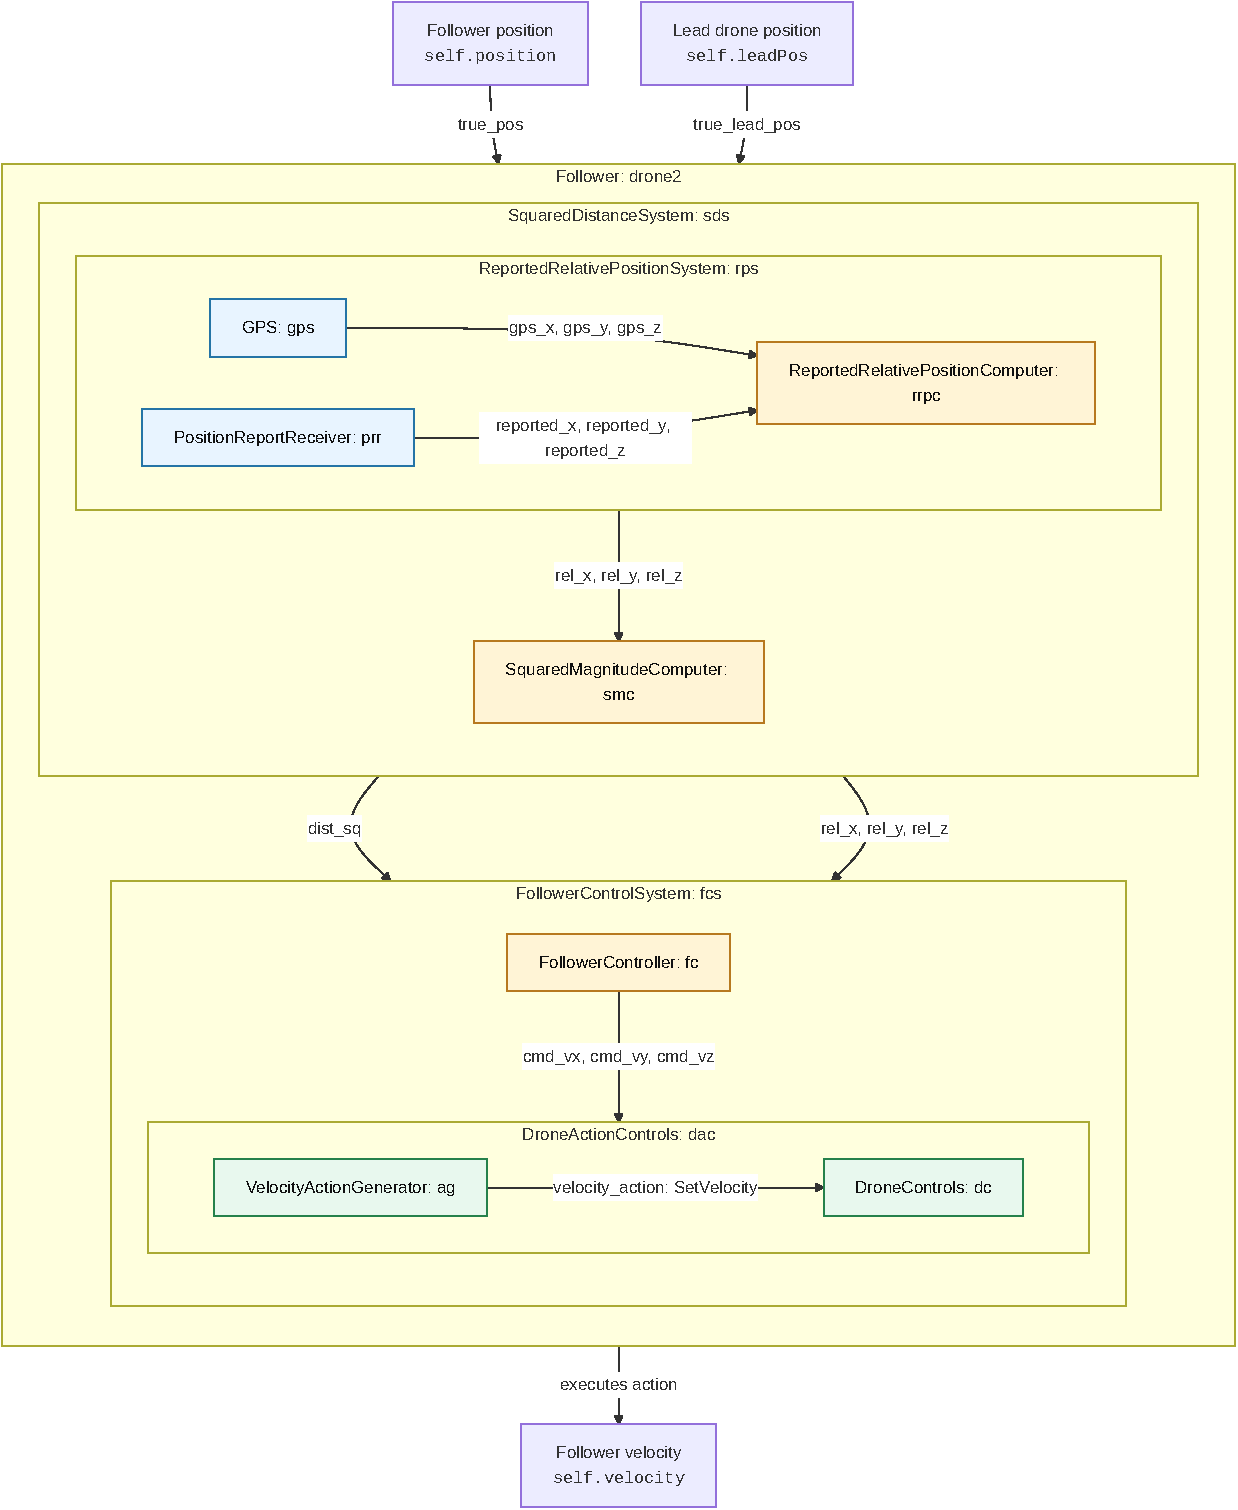
\includegraphics[width=0.78\textwidth,height=0.72\textheight,keepaspectratio]
        {figures/drone_distance_diagrams-2.pdf}
    \caption{Composition and data flow of the follower implementation.}
    \label{fig:component-data-flow}
\end{figure}

\section{Idea}
The contract describes a scenario with two quadcopter drones, Leader and Follower. The Leader drone behavior is taken from the patrol example in \verb|followPatrol.scenic|. The Follower drone behavior is initialized there with the \texttt{Follow} behavior, but then overridden by a compositional implementation in \verb|drone_distance.contract|.

The Leader does the Patrol behavior, which is just going around the environment slowly. The Follower starts 100 units away, and must get close to the Leader, but not too close, and continue to stay within a certain range as best as possible.

This corresponds to four verified end-to-end results: a progress property, a
simulation-tested liveness property, directional movement safety, and a
never-crash invariant with a positive separation floor.

The minimum and maximum follow distances are $5$ and $15$. The approach gain is
$0.2$, the retreat gain is $0.5$, the maximum velocity in each component is $3$,
the maximum Leader speed is $2$, and the simulation timestep is $0.1$ seconds.

\section{Components}

\subsection{\texttt{GPS}}

\paragraph{Sensors.}
\begin{itemize}
    \item \verb|self.position|, exposed internally as \verb|true_pos| (\verb|Vector|)
\end{itemize}

\paragraph{Inputs.} None.

\paragraph{Outputs.}
\begin{itemize}
    \item \verb|gps_x|, \verb|gps_y|, \verb|gps_z| (\verb|float|)
\end{itemize}

\paragraph{Description.} This component reports the exact position of the Follower.

\subsection{\texttt{PositionReportReceiver}}

\paragraph{Sensors.}
\begin{itemize}
    \item \verb|self.leadPos|, exposed internally as \verb|true_lead_pos| (\verb|Vector|)
\end{itemize}

\paragraph{Inputs.} None.

\paragraph{Outputs.}
\begin{itemize}
    \item \verb|reported_x|, \verb|reported_y|, \verb|reported_z| (\verb|float|)
\end{itemize}

\paragraph{Description.} This component receives and outputs the (exact) position as ``reported'' by the Leader. Together with the \texttt{GPS} component, it models ideal sensing: positions are available without noise, error, or delay.

\subsection{\texttt{ReportedRelativePositionComputer}}

\paragraph{Inputs.}
\begin{itemize}
    \item \verb|own_x|, \verb|own_y|, \verb|own_z| (\verb|float|)
    \item \verb|reported_x|, \verb|reported_y|, \verb|reported_z| (\verb|float|)
\end{itemize}

\paragraph{Outputs.}
\begin{itemize}
    \item \verb|rel_x|, \verb|rel_y|, \verb|rel_z| (\verb|float|)
\end{itemize}

\paragraph{Description.} This component computes the relative position of the Leader from the Follower. Given that the Leader is at position $\hat r_\ell$ and the Follower is at position $\hat r_f$, it returns $\hat r_\ell - \hat r_f$.

\subsection{\texttt{ReportedRelativePositionSystem}}

\paragraph{Inputs.} None.

\paragraph{Outputs.}
\begin{itemize}
    \item \verb|rel_x|, \verb|rel_y|, \verb|rel_z| (\verb|float|)
\end{itemize}

\paragraph{Composition.}
See Figure~\ref{fig:component-data-flow}.
\begin{itemize}
    \item \verb|gps|: \verb|GPS|
    \item \verb|prr|: \verb|PositionReportReceiver|
    \item \verb|rrpc|: \verb|ReportedRelativePositionComputer|
\end{itemize}
The subcomponents are connected as follows:
\begin{itemize}
    \item \verb|gps.gps_x|, \verb|gps.gps_y|, and \verb|gps.gps_z| connect to
          \verb|rrpc.own_x|, \verb|rrpc.own_y|, and \verb|rrpc.own_z|, respectively.
    \item \verb|prr.reported_x|, \verb|prr.reported_y|, and
          \verb|prr.reported_z| connect to \verb|rrpc.reported_x|,
          \verb|rrpc.reported_y|, and \verb|rrpc.reported_z|, respectively.
    \item \verb|rrpc.rel_x|, \verb|rrpc.rel_y|, and \verb|rrpc.rel_z| connect
          to the corresponding outputs of the system.
\end{itemize}

\paragraph{Description.} This component gets the Follower's position and the Leader's position from its internal sensor components and asks the \texttt{ReportedRelativePositionComputer} for the relative position vector, then outputs that vector. 

\subsection{\texttt{SquaredMagnitudeComputer}}

\paragraph{Inputs.}
\begin{itemize}
    \item \verb|rel_x|, \verb|rel_y|, \verb|rel_z| (\verb|float|)
\end{itemize}

\paragraph{Outputs.}
\begin{itemize}
    \item \verb|dist_sq| (\verb|float|)
\end{itemize}

\paragraph{Description.} This component computes the squared magnitude of a vector.

\subsection{\texttt{SquaredDistanceSystem}}

\paragraph{Inputs.} None.

\paragraph{Outputs.}
\begin{itemize}
    \item \verb|dist_sq| (\verb|float|)
    \item \verb|rel_x|, \verb|rel_y|, \verb|rel_z| (\verb|float|)
\end{itemize}

\paragraph{Composition.}
See Figure~\ref{fig:component-data-flow}.
\begin{itemize}
    \item \verb|rps|: \verb|ReportedRelativePositionSystem|
    \item \verb|smc|: \verb|SquaredMagnitudeComputer|
\end{itemize}
The subcomponents are connected as follows:
\begin{itemize}
    \item \verb|rps.rel_x|, \verb|rps.rel_y|, and \verb|rps.rel_z| connect both
          to the corresponding outputs of the system and to \verb|smc.rel_x|,
          \verb|smc.rel_y|, and \verb|smc.rel_z|, respectively.
    \item \verb|smc.dist_sq| connects to the \verb|dist_sq| output of the system.
\end{itemize}

\paragraph{Description.} This component combines the two preceding systems. It gets the relative position from the former and asks the latter for the squared magnitude of that vector, then outputs \textit{both} the vector and its squared magnitude. 

\subsection{\texttt{FollowerController}}

\paragraph{Parameters.}
\begin{itemize}
    \item \verb|min_dist|, \verb|max_dist|, \verb|gain|,
          \verb|retreat_gain|, \verb|max_component_speed|
\end{itemize}

\paragraph{Inputs.}
\begin{itemize}
    \item \verb|dist_sq| (\verb|float|)
    \item \verb|rel_x|, \verb|rel_y|, \verb|rel_z| (\verb|float|)
\end{itemize}

\paragraph{Outputs.}
\begin{itemize}
    \item \verb|cmd_vx|, \verb|cmd_vy|, \verb|cmd_vz| (\verb|float|)
\end{itemize}

\paragraph{Description.} This component takes as input the relative position vector and its squared magnitude, then uses the information to decide with what velocity the Follower should move. 

The decision depends on the (squared) distance to the Leader. The component takes as parameters a minimum and maximum distance which determine a spherical shell (a ``band'') centered around the Leader. If the distance from the Follower to the Leader is greater than the outer radius of the band, the Follower moves closer. If it is less than the inner radius, the Follower retreats. At either boundary or within the band, the Follower hovers.\footnote{Hovering was broken for a while: whenever the controller commanded a velocity of zero, the Follower would sink to the ground and only recover after hitting it. The hover logic was actually fine---the bug was in the conversion from Scenic velocities to AirSim. We were routing velocities through the \emph{location} converters, which apply the world offset and a $\times 100$ mesh scaling, so with \texttt{worldOffset} $= (0, 0, 50)$ a commanded $(0,0,0)$ came out as $(0, 0, 0.5)$: a constant $0.5$ m/s downward push every time the Follower was told to stop. And because the location path never flips the $z$-axis (Scenic is $z$-up, AirSim's NED frame is $z$-down), corrective climbs were delivered as further descent, so the drone couldn't recover until the ground stopped it. The fix was to give velocities their own axis-only converters (no offset, no scaling, correct sign), rather than to special-case the hover.}

The magnitude\footnote{Strictly speaking the direction too: because we clamp each coordinate independently rather than scaling the vector uniformly (this just makes the Lean/math easier), the clamped velocity need not point exactly along $\hat r_\ell - \hat r_f$. What survives is that each component keeps its sign, so the motion still points into the correct octant—toward the Leader when approaching, away when retreating. This is what the directional-safety contract establishes.} of the commanded velocity depends on the component-wise distance between the two drones and three parameters: \texttt{max\_component\_speed}, \texttt{gain}, and \texttt{retreat\_gain}.

The first parameter, \texttt{max\_component\_speed}, ensures that the Follower is never commanded to move too fast. Write $M = \texttt{max\_component\_speed}$. Each component $v$ is clamped to the interval $[-M,M]$ using $\min(\max(v,-M),M)$. Thus the commanded speed is never greater than $M\sqrt{3}$. The parameter \texttt{gain} controls the proportional approach response outside the outer boundary. The separate \texttt{retreat\_gain} controls the proportional retreat response inside the inner boundary.

\subsection{\texttt{VelocityActionGenerator}}

\paragraph{Inputs.}
\begin{itemize}
    \item \verb|cmd_vx|, \verb|cmd_vy|, \verb|cmd_vz| (\verb|float|)
\end{itemize}

\paragraph{Outputs.}
\begin{itemize}
    \item \verb|velocity_action| (\verb|SetVelocity|)
\end{itemize}

\paragraph{Description.} This component takes in a commanded velocity and turns it into a \texttt{SetVelocity}, which is an AirSim-specific way of telling a drone to start moving with a certain velocity. 

\subsection{\texttt{DroneControls}}

\paragraph{Inputs.} None.

\paragraph{Outputs.} None.

\paragraph{Actions.}
\begin{itemize}
    \item \verb|velocity_action| (\verb|SetVelocity|)
\end{itemize}

\paragraph{Description.} This component receives the action produced by the \texttt{VelocityActionGenerator} and ``actually'' executes it. 

\subsection{\texttt{DroneActionControls}}

\paragraph{Inputs.}
\begin{itemize}
    \item \verb|cmd_vx|, \verb|cmd_vy|, \verb|cmd_vz| (\verb|float|)
\end{itemize}

\paragraph{Outputs.} None.

\paragraph{Composition.}
See Figure~\ref{fig:component-data-flow}.
\begin{itemize}
    \item \verb|ag|: \verb|VelocityActionGenerator|
    \item \verb|dc|: \verb|DroneControls|
\end{itemize}
The subcomponents are connected as follows:
\begin{itemize}
    \item The system inputs \verb|cmd_vx|, \verb|cmd_vy|, and \verb|cmd_vz|
          connect to the corresponding inputs of \verb|ag|.
    \item \verb|ag.velocity_action| connects to \verb|dc.velocity_action|.
\end{itemize}

\paragraph{Description.} This component composes the two subcomponents listed above. It receives the commanded velocity from the controller, passes it to the action generator, and then passes the resulting action to the drone controls, which execute it.

\subsection{\texttt{FollowerControlSystem}}

\paragraph{Parameters.}
\begin{itemize}
    \item \verb|min_dist|, \verb|max_dist|, \verb|gain|,
          \verb|retreat_gain|, \verb|max_component_speed|
\end{itemize}

\paragraph{Inputs.}
\begin{itemize}
    \item \verb|dist_sq| (\verb|float|)
    \item \verb|rel_x|, \verb|rel_y|, \verb|rel_z| (\verb|float|)
\end{itemize}

\paragraph{Outputs.} None.

\paragraph{Composition.}
See Figure~\ref{fig:component-data-flow}.
\begin{itemize}
    \item \verb|fc|: \verb|FollowerController|, instantiated with the five
          parameters listed above
    \item \verb|dac|: \verb|DroneActionControls|
\end{itemize}
The subcomponents are connected as follows:
\begin{itemize}
    \item The system inputs \verb|dist_sq|, \verb|rel_x|, \verb|rel_y|, and
          \verb|rel_z| connect to the corresponding inputs of \verb|fc|.
    \item \verb|fc.cmd_vx|, \verb|fc.cmd_vy|, and \verb|fc.cmd_vz| connect to
          \verb|dac.cmd_vx|, \verb|dac.cmd_vy|, and \verb|dac.cmd_vz|,
          respectively.
\end{itemize}

\paragraph{Description.} This component takes the relative position vector and its squared magnitude and passes them to the \texttt{FollowerController}, which uses them to compute the commanded velocity. It then passes that velocity to the \texttt{DroneActionControls}, which turns it into an action and executes it.

\subsection{\texttt{Follower}}

\paragraph{Parameters.}
\begin{itemize}
    \item \verb|min_dist|, \verb|max_dist|, \verb|gain|,
          \verb|retreat_gain|, \verb|max_component_speed| (\verb|float|)
\end{itemize}

\paragraph{Inputs.} None.

\paragraph{Outputs.} None.

\paragraph{Composition.}
See Figure~\ref{fig:component-data-flow}.
\begin{itemize}
    \item \verb|sds|: \verb|SquaredDistanceSystem|
    \item \verb|fcs|: \verb|FollowerControlSystem|, instantiated with the five
          parameters listed above
\end{itemize}
The subcomponents are connected as follows:
\begin{itemize}
    \item \verb|sds.dist_sq| connects to \verb|fcs.dist_sq|.
    \item \verb|sds.rel_x|, \verb|sds.rel_y|, and \verb|sds.rel_z| connect to
          \verb|fcs.rel_x|, \verb|fcs.rel_y|, and \verb|fcs.rel_z|,
          respectively.
\end{itemize}

\paragraph{Description.} This is the whole Follower drone! It is made up of the \texttt{SquaredDistanceSystem} which is like the perception system from the car example and the \texttt{FollowerControlSystem} which is a composite of the control system and the actuator from the car example.

\section{Contracts}

\subsection{Position and Distance Contracts}

\subsubsection{\texttt{GPSAccurate}}

\paragraph{Kind.} Assumption on the \texttt{GPS} component.

\paragraph{Description.} This is a simple assumption that the ``GPS'' component is accurate; i.e. the position it reports is exactly equal to the actual position of the Follower.

\subsubsection{\texttt{PositionReportReceiverAccurate}}

\paragraph{Kind.} Assumption on the \texttt{PositionReportReceiver} component.

\paragraph{Description.} This is the analogous assumption on the Leader's ``GPS'' and reporting: it codifies the assumption that the Leader knows its own position accurately and reports it to the Follower accurately.

\subsubsection{\texttt{ReportedRelativePositionComputerSemantics}}

\paragraph{Kind.} Proved directly about the \texttt{ReportedRelativePositionComputer} component.

\paragraph{Description.} This is a contract that states the relative position is computed correctly as the component-wise difference of the Leader's position and the Follower's position. 

\subsubsection{\texttt{ReportedRelativePositionAccurate}}

\paragraph{Kind.} Refinement of the contracts for the GPS, position report receiver, and relative position computer composed over the \texttt{ReportedRelativePositionSystem}.

\paragraph{Description.} This is a refinement of the composite of the above three contracts: it states that the computed relative position is equal to the difference of the actual positions of the two drones, not just the reported positions. 

\subsubsection{\texttt{SquaredMagnitudeComputerSemantics}}

\paragraph{Kind.} Proved directly about the \texttt{SquaredMagnitudeComputer} component.

\paragraph{Description.} This states that the squared magnitude of the relative position (or really whatever vector the \texttt{SquaredMagnitudeComputer} receives) is in fact the squared magnitude of that vector. 

\subsubsection{\texttt{SquaredDistanceSystemAccuracy}}

\paragraph{Kind.} Refinement over the \texttt{SquaredDistanceSystem} using the two contracts above.

\paragraph{Description.} This is a refinement of the above two which combines the two guarantees exactly into one contract. 

\subsection{Controller and Actuation Contracts}

\subsubsection{\texttt{FollowerControllerSemantics}}

\paragraph{Kind.} Proved directly about the \texttt{FollowerController} component.

\paragraph{Description.} Under sensible assumptions on the parameters (for example, both gains are positive and the band is not inverted), this contract states the following:
\begin{itemize}
    \item Whenever the Follower is inside the band, its commanded velocity is zero.
    \item Outside the band, the commanded velocity equals the component's clamped proportional response: \texttt{gain} for approach and \texttt{retreat\_gain} for retreat.
\end{itemize}

\paragraph{Assumptions.} Both gains and the maximum component speed are
positive, $0 \leq \texttt{min\_dist} \leq \texttt{max\_dist}$.

\subsubsection{\texttt{FollowerControllerDirectionalSafety}}

\paragraph{Kind.} Refinement of \texttt{FollowerControllerSemantics}.

\paragraph{Description.} This is a refinement of the above into a strictly weaker but still necessary guarantee on the Follower's behavior. It states that the follower is always pointed in the ``right'' direction, i.e. if it is too far away, the dot product of the commanded velocity and position vectors is positive (so it moves towards the Leader) and if it is too close the dot product is negative (so it moves away). 

This contract also states (componentwise) the $\sqrt3 M$ bound on the commanded velocity. 

\subsubsection{\texttt{VelocityActuation}}

\paragraph{Kind.} Assumption on the \texttt{DroneActionControls} component, with correctness $0.99$ and confidence $0.999$.

\paragraph{Description.} We assume that the velocity actuator provided by AirSim works as intended with the stated correctness and confidence. 

\subsubsection{\texttt{FollowerVelocityDirectionalSafety}}

\paragraph{Kind.} Refinement over the \texttt{FollowerControlSystem} using the directional controller and actuation contracts above.

\paragraph{Description.} This is a refinement over the previous contract which makes the same claims about the \textit{actual} next velocity of the drone, rather than about the commanded velocity (which we assumed with small probability may not have been executed correctly). 

\subsubsection{\texttt{FollowerVelocitySemantics}}

\paragraph{Kind.} Refinement over the \texttt{FollowerControlSystem} using the exact controller semantics and actuation contracts above.

\paragraph{Description.} This does the same as the above but for the exact equality claims in \texttt{FollowerControllerSemantics}.

In particular, the next velocity is zero inside the band, uses \texttt{gain} in
the approach branch, and uses \texttt{retreat\_gain} in the retreat branch.

\subsection{End-to-End Contracts}

\subsubsection{\texttt{KeepsFollowDistanceProgress}}

\paragraph{Kind.} Refinement of \texttt{FollowerVelocitySemantics} and \texttt{SquaredDistanceSystemAccuracy} composed over the complete Follower.

\paragraph{Description.} This contract says that if the Follower is too far away, it is guaranteed to get closer to the Leader in the next step.

\paragraph{Assumptions.} The parameters are positive, position follows the
velocity integration law with timestep $0.1$, and the Leader moves at most $0.2$
units per step. Above the outer boundary, the Follower's minimum approach speed
is greater than the Leader's maximum speed.

\subsubsection{\texttt{KeepsFollowDistanceLiveness}}

\paragraph{Kind.} Tested directly on the complete Follower using simulation.

\paragraph{Description.} This is the tested half of the liveness guarantee, which says that the Follower eventually gets inside the outer ring of the band around the Leader.

The contract is tested on the complete Follower in the AirSim patrol scenario.
Each simulation runs for at most $600$ steps. Testing uses confidence $0.999$, a
batch size of $1$, NumPy seed $42$, and a five-minute testing time budget.

\subsubsection{\texttt{FollowerMovementDirectionalSafety}}

\paragraph{Kind.} Refinement of \texttt{FollowerVelocityDirectionalSafety} and \texttt{SquaredDistanceSystemAccuracy} composed over the complete Follower.

\paragraph{Description.} This says that the Follower's actual step always points the right way: when it is too far, the step's dot product with the true relative position comes out non-negative, so it moves toward the Leader; when it is too close, the dot product is non-positive, so it moves away. It is worth being clear that this is only about direction --- it pins down the sign of a single step, not what the distance does over time, so on its own it does not rule out a collision. That is what \texttt{NeverCrash} is for.

\paragraph{Assumptions.} The follow-distance band is not inverted, and position
follows the velocity integration law with the configured timestep of $0.1$.

\subsubsection{\texttt{NeverCrash}}

\paragraph{Kind.} Refinement over the complete Follower. It composes
\texttt{FollowerVelocitySemantics}, which gives the exact velocity semantics,
with \texttt{SquaredDistanceSystemAccuracy}.

\paragraph{Description.} This is the one that says the Follower never crashes
into the Leader: the true distance always stays above a positive floor $R$. The
floor is what is left of the inner radius once the Leader has taken its one step
toward the Follower, $R = \texttt{min\_dist} -
\texttt{max\_leader\_speed}\cdot\texttt{timestep}$, and the guarantee is
\[
    \texttt{always}\quad \texttt{true\_dist\_sq} \geq R^2.
\]
This rests on two assumptions: that the Leader cannot cover the whole inner
radius in a single step (so the floor stays positive), and that an approach step
from outside the band cannot overshoot the floor. Both are satisfied by the
configured values --- the floor works out to $R = 4.8$, and the no-overshoot
condition needs $\texttt{max\_dist} \geq 5.9$ against the actual $15$.

\paragraph{Assumptions.} The parameters and collision floor are positive. The
Follower starts at or above the floor, position follows the velocity integration
law, and the Leader's displacement is bounded by its maximum speed. Throughout
the retreat region, the retreat speed is at least the Leader's maximum speed and
the velocity clamp is inactive. An approach step from beyond the outer boundary
cannot cross the floor.

\begin{figure}[H]
    \centering
    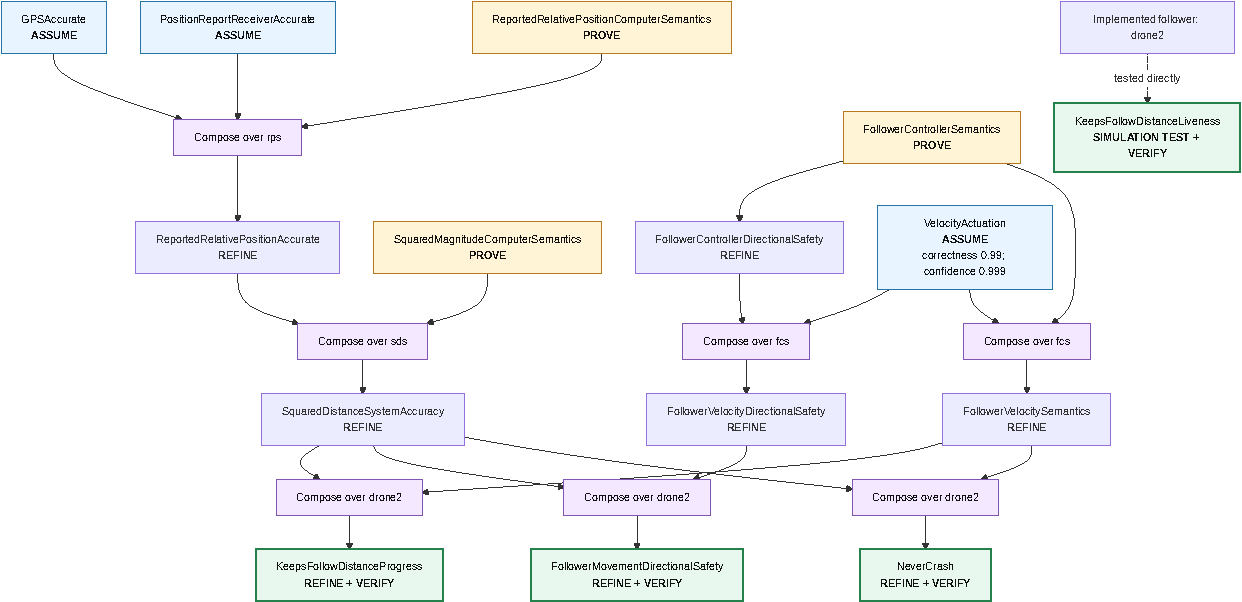
\includegraphics[width=0.95\textwidth,height=0.78\textheight,keepaspectratio]
        {figures/drone_distance_diagrams-4.pdf}
    \caption{Contract composition, proof, refinement, and verification structure.}
    \label{fig:contract-composition}
\end{figure}

\begin{figure}[H]
    \centering
    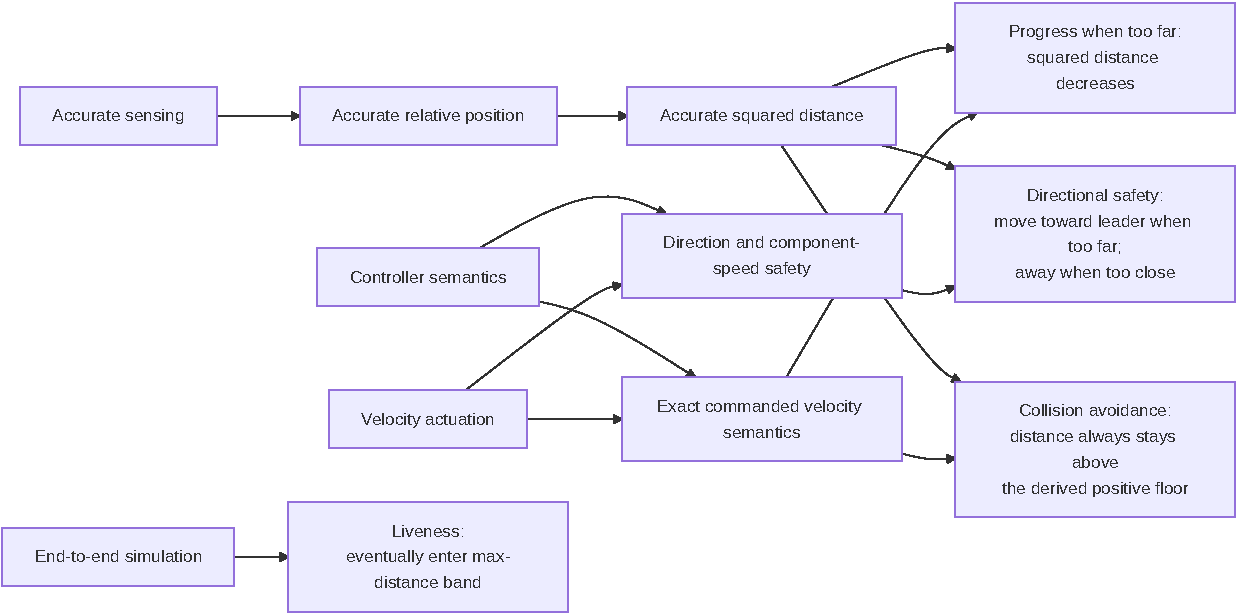
\includegraphics[width=\textwidth]{figures/drone_distance_diagrams-5.pdf}
    \caption{Summary of the properties established by the contracts.}
    \label{fig:contract-results}
\end{figure}

\end{document}
